\documentclass{beamer}
\usefonttheme{serif}

\usepackage{multicol}

\beamertemplatenavigationsymbolsempty

\usepackage{fontspec}
\usepackage{pgfpages}
\usepackage{tikz}
\usetikzlibrary{arrows}
\usetikzlibrary{shapes.misc}
\tikzset{
  invisible/.style={opacity=0},
  visible on/.style={alt={#1{}{invisible}}},
  alt/.code args={<#1>#2#3}{%
    \alt<#1>{\pgfkeysalso{#2}}{\pgfkeysalso{#3}} % \pgfkeysalso doesn't change the path
  },
}

\setsansfont{Josefin Sans}
\setmainfont{Josefin Slab}

\definecolor{accentcol}{HTML}{0C4502} % cs452 css colour ;)
\setbeamercolor{structure}{fg=accentcol}
\setbeamertemplate{navigation symbols}{}

\usetheme{Bergen}

\title{Fuzzy Logic and Neural Networks in CS452}
\author{Louis Burke}
\logo{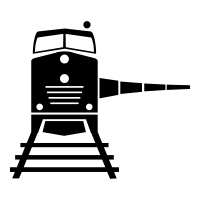
\includegraphics[scale=0.1]{train}}

\begin{document}

\frame{\titlepage}

\begin{frame}{The AI Problem}
	\begin{itemize}
		\item Approximate the real world in software.
		\item Analogously approximate a function.
		\item 5 common solutions: \begin{enumerate}
			\item Heuristics
			\item Genetics
			\item Fuzzy Logic
			\item Neural Network
		\end{enumerate}
		\item Worthy mentions: \begin{enumerate}
			\item Distributed (we only have 1 system)
			\item Cooperative (still just 1 system)
			\item Adaptive (I haven't learnt it, but probably very effective)
		\end{enumerate}
	\end{itemize}
\end{frame}

\begin{frame}{Heuristics and Genetics}
	Heuristics:

	\begin{itemize}
		\item Requires accurate modelling
		\item Difficult to extend
		\item Cannot learn
		\item Easiest to inspect and debug
	\end{itemize}

	Genetics:

	\begin{itemize}
		\item Learns too slow!
	\end{itemize}
\end{frame}

\begin{frame}{Genetics}
	\begin{itemize}
		\item Learns too slow!
	\end{itemize}
\end{frame}

\begin{frame}{Fuzzy vs Neural}
	\begin{tabular}{c|c|c}
		& Fuzzy Logic & Neural Networks \\ \hline
		Best suited for & Control & Classification \\
		Speed & Fast & Slow \\
		Programming & Manual & Automatic \\
		Learning & No & Yes \\
		Requirements & Rules & Data
	\end{tabular}
\end{frame}

\begin{frame}{Fuzzy Logic Basics}
	\begin{itemize}
		\item First turn inputs into fuzzy variables
		\item Then do logic with those variables
		\item Then turn fuzzy variables back to outputs
	\end{itemize}
\end{frame}

\begin{frame}{Fuzzification}
	\begin{itemize}
		\item Fuzzy sets have non-integer inclusion
		\item In crisp sets: $x \in S$ is boolean
		\item In fuzzy sets: $x \in S$ is an element from another set (usually reals)
		\item Typical membership functions:
	\end{itemize}

	\begin{multicols}{2}
		\center{Trapezoidal}
		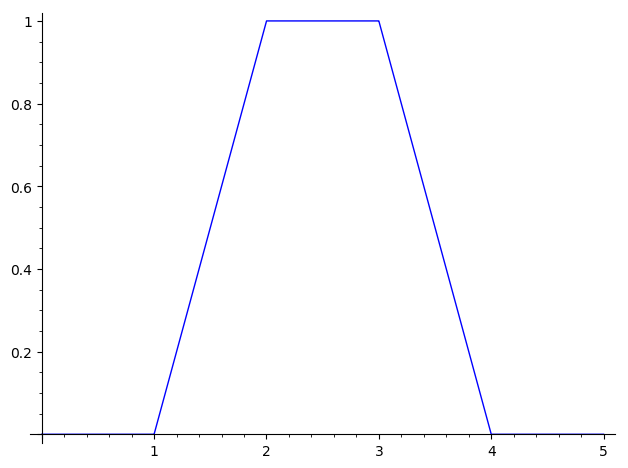
\includegraphics[width=0.5\textwidth]{trapezoidal}
		\center{Bell}
		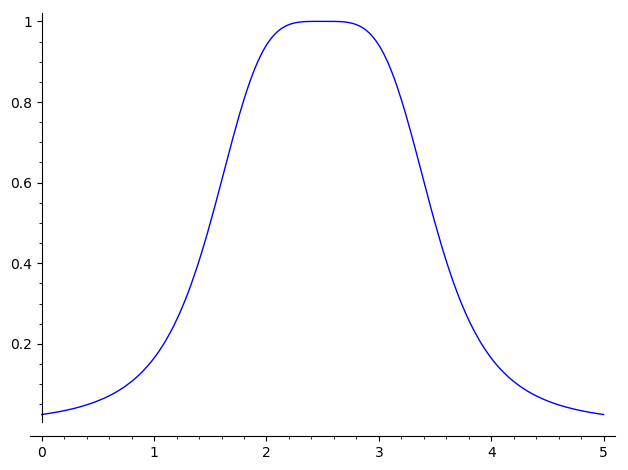
\includegraphics[width=0.5\textwidth]{bell}
	\end{multicols}
\end{frame}

\begin{frame}{Fuzzifier Comparison}
	\begin{tabular}{c|c}
		Trapezoidal & Bell \\ \hline
		Faster & Slower \\
		Not Differentiable & Differentiable \\
		Less accurate & More accurate
	\end{tabular}

	Importance of differentiability is it allows the use of gradient descent
	algorithms on the membership functions.
\end{frame}

\begin{frame}{Fuzzy T-norm}
	\begin{itemize}
		\item Fuzzy equivalent to AND operation
		\item Comes with the equivalent S-norm (OR)
		\item S-norm computed via DeMorgan
		\item Typical T-norms:
	\end{itemize}

	\begin{multicols}{4}
		\center{Classical}
		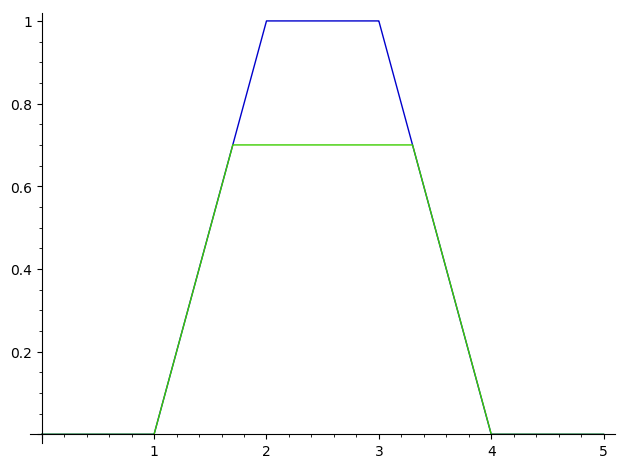
\includegraphics[width=0.25\textwidth]{classical_tnorm}
		\center{Algebraic}
		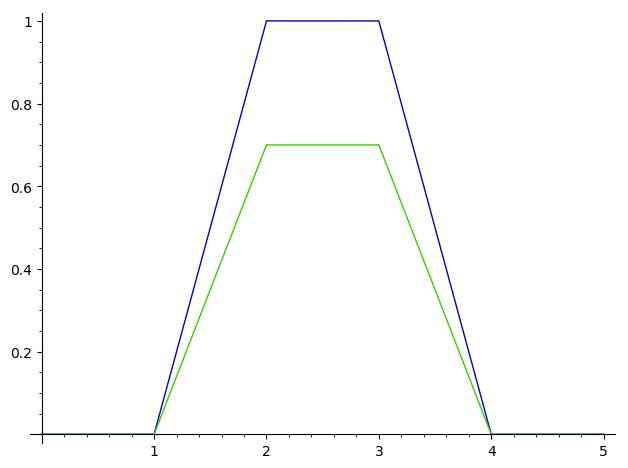
\includegraphics[width=0.25\textwidth]{algebraic_tnorm}
		\center{Bounded}
		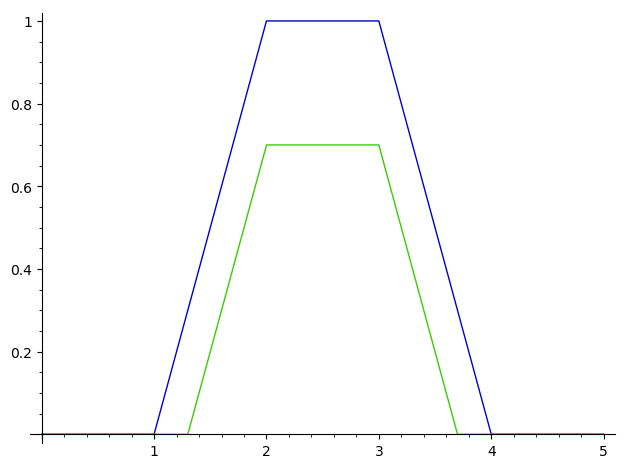
\includegraphics[width=0.25\textwidth]{bounded_tnorm}
		\center{Basic}
		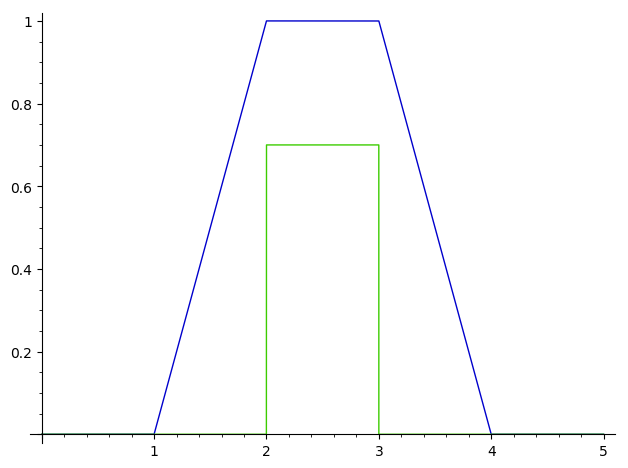
\includegraphics[width=0.25\textwidth]{basic_tnorm}
	\end{multicols}
\end{frame}

\begin{frame}{Fuzzy Implications}
	Like T-norm, not obvious. Common implication schemes:

	\begin{multicols}{5}
		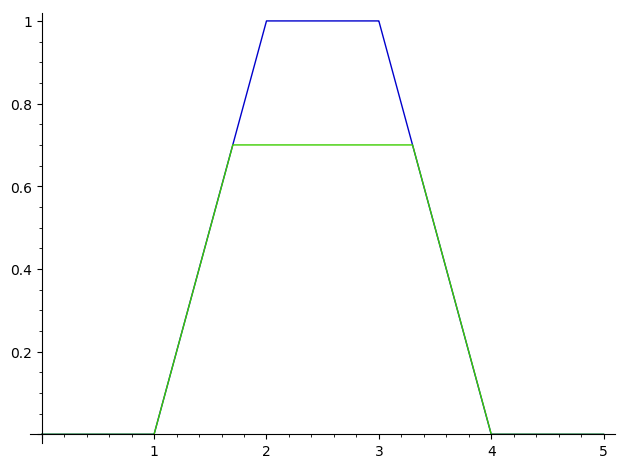
\includegraphics[width=0.2\textwidth]{mamdani}
		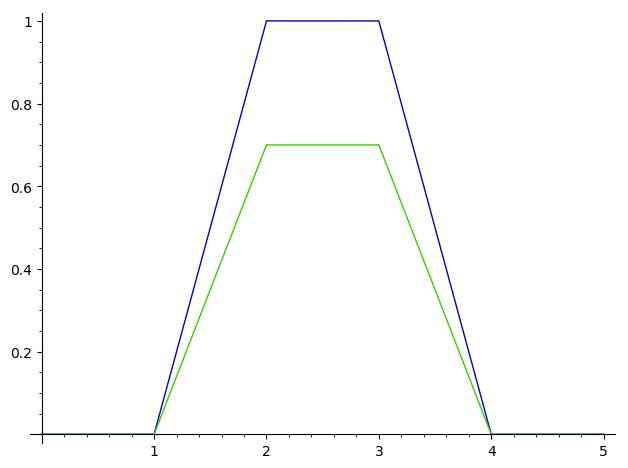
\includegraphics[width=0.2\textwidth]{larsen}
		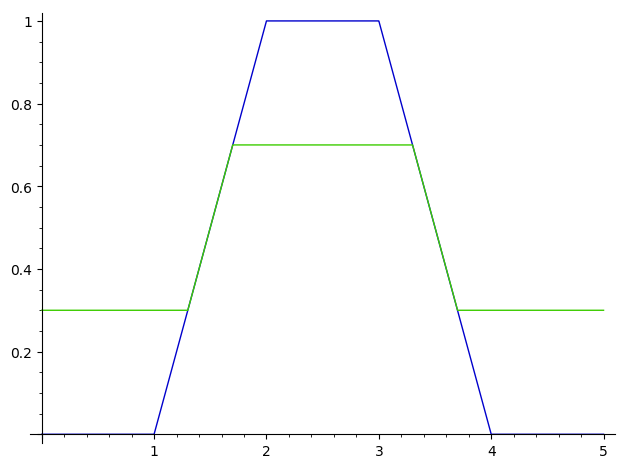
\includegraphics[width=0.2\textwidth]{zadeh}
		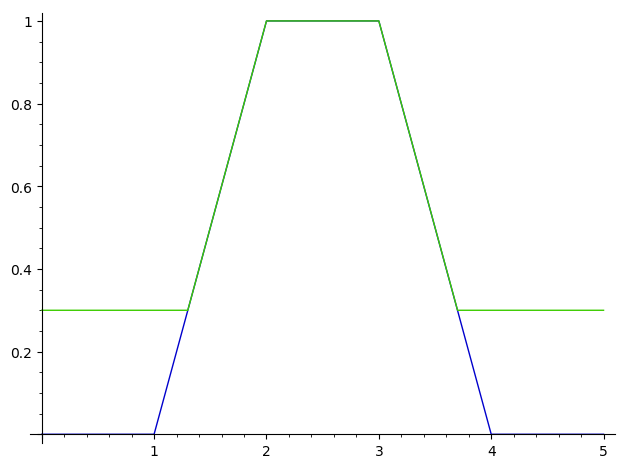
\includegraphics[width=0.2\textwidth]{dr}
		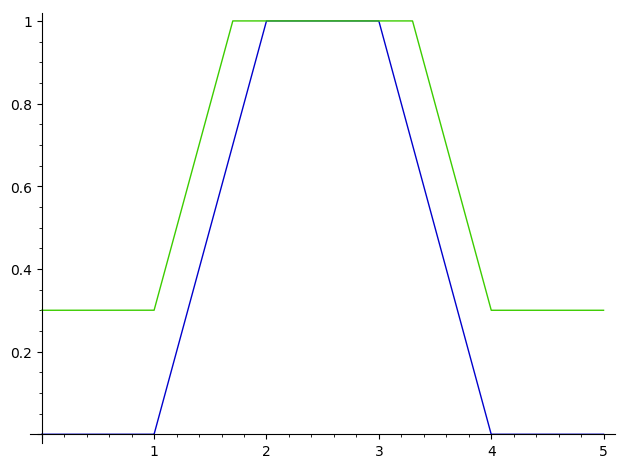
\includegraphics[width=0.2\textwidth]{luke}
	\end{multicols}

	From left to right: Mamdani, Larsen, Zadeh, Dienes-Rascher, Lukasiewicz.
\end{frame}

\begin{frame}{Defuzzification}
	Last fuzzy operation, turn fuzzy back to non-fuzzy. Common defuzzification
	schemes:

	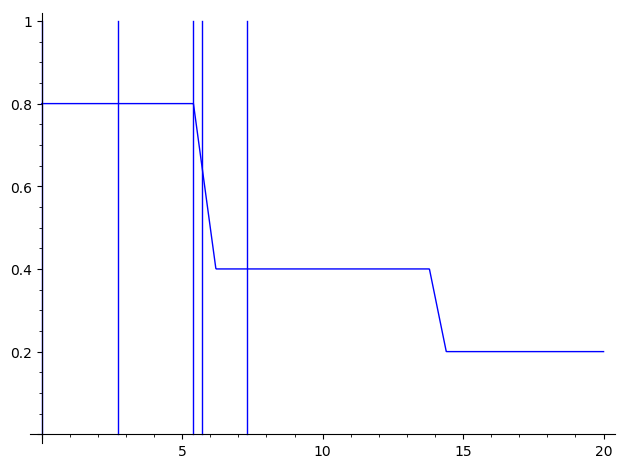
\includegraphics[width=\textwidth]{defuz}

	From left to right: Min of max (at 0), Mean of max, Max of max, Center of
	area, Centroid.
\end{frame}

% TODO: basic intro to neural networks too
% Emphasize that nn's find PATTERNS!

\begin{frame}{Recommendations}
	\begin{itemize}
		\item Use a neural network to learn how long it takes a train to get
from switch to switch.
		\item If that is too slow, simply save last switch-to-switch time?
		\item Take time since last switch, expected switch-to-switch time,
speed, etc to fuzzily determine location.
		\item Definitely look into adaptive algorithms (especially
Least-Mean-Squares) to possibly swap out for the neural network.
	\end{itemize}
\end{frame}

\end{document}

% NN for ETA at next switch. Time/ETA as input to Fuzzy!
% Fuzzy also deals with speed changes/acceleration


